% ****** Start of file .tex ******
%
%   This file is based on apssamp.tex, part of the APS files in the REVTeX 4.1 distribution.
%   Version 4.1r of REVTeX, August 2010
%
%   Copyright (c) 2009, 2010 The American Physical Society.
%   Samuel Balula, Pedro Ribeiro, Luís Macedo, Eduardo Neto 2013
%   See the REVTeX 4 README file for restrictions and more information.
%
% TeX'ing this file requires that you have AMS-LaTeX 2.0 installed
% as well as the rest of the prerequisites for REVTeX 4.1
%
% See the REVTeX 4 README file
% It also requires running BibTeX. The commands are as follows:
%
%  1)  latex filename.tex
%  2)  bibtex filename
%  3)  latex filename.tex
%  4)  latex filename.tex

\documentclass[%
  reprint,
  %superscriptaddress,
  %groupedaddress,
  %unsortedaddress,
  %runinaddress,
  %frontmatterverbose, 
  %preprint,
  %showpacs,preprintnumbers,
  nofootinbib,
  %nobibnotes,
  %bibnotes,
  amsmath,amssymb,
  aps,
  %pra,
  %prb,
  %rmp,
  %prstab,
  %prstper,
  %floatfix,
  10pt,
  a4paper
]{revtex4-1}



\usepackage{facil}                      % Pacote pessoal
\usepackage{verbatim}                   % Apresentação de código
\usepackage{graphicx}                   % Include figure files
\usepackage{dcolumn}                    % Align table columns on decimal point
\usepackage{bm}                         % bold math
\usepackage[latin1,utf8]{inputenc}      % Tipos de caracteres
\usepackage[portuges]{babel}            % Português
\usepackage{indentfirst}                % Identação da primeira linha
\usepackage{hyperref}                   % add hypertext capabilities
\usepackage{float}                      %Fixar imagens
\usepackage{multirow}
%\usepackage[mathlines]{lineno}          % Enable numbering of text and display math
%\linenumbers\relax                      % Commence numbering lines
%\usepackage[compact]{titlesec}

\usepackage[%showframe,%Uncomment any one of the following lines to test 
%%scale=0.7, marginratio={1:1, 2:3}, ignoreall, % default settings
%%text={7in,10in},centering,
margin=0.5in,        %diminuir margens
%total={6.5in,8.75in}, top=1.2in, left=0.9in, 
includefoot
%height=10in,a5paper,hmargin={3cm,0.8in},
]{geometry}

\begin{document}
\preprint{APS/123-QED}
%\captionsetup[table]{font=small,skip=0pt}
%\captionsetup[figure]{font=small,skip=0pt}
%\titlespacing{\section}{0pt}{*0}{*0}            %Poupar espaço
%\titlespacing{\subsection}{0pt}{*0}{*0}
%\titlespacing{\subsubsection}{0pt}{*0}{*0}


% % % % % % % % % % % % % % % % % % % % % % % % % % % % % % % % % % % % % % % % 
%%%%%%%%%%%%%%%%%%%%%%%%%%%%%%%%%% Início %%%%%%%%%%%%%%%%%%%%%%%%%%%%%%%%%%%%%%
% % % % % % % % % % % % % % % % % % % % % % % % % % % % % % % % % % % % % % % %
 

\title{Andar final de amplificação em classe A\\
com transistores bipolares 2n3055}
\thanks{}

\author{Pedro Ribeiro}%
\email{73221, pedro.q.ribeiro@tecnico.ulisboa.pt}
\author{Luis Macedo}%
\email{73633, luis.macedo@tecnico.ulisboa.pt}
\author{Samuel Balula}%
\email{72735, samuel.balula@tecnico.ulisboa.pt}

\affiliation{
  Instituto Superior Técnico\\
  Mestrado em Engenharia Física Tecnológica\\
  Complementos de Electrónica
}

%\collaboration{Grupo 57}

\date{\today}

%%%%%%%%%%%%%%%%%%%%%%%%%%%%%%%%%% Abstract %%%%%%%%%%%%%%%%%%%%%%%%%%%%%%%%%%%%
\begin{abstract}

\end{abstract}
\maketitle


%%%%%%%%%%%%%%%%%%%%%%%%%%%%%%%%%% Introdução %%%%%%%%%%%%%%%%%%%%%%%%%%%%%%%%%%
\section{Introdução}
\label{s:intro}
%Situar o problema, incluir fórmulas.
%Quem lê o relatório deve conseguir perceber exatamente o que foi feito.

Analisando o circuito do andar de saída em classe A obtém-se, através das equações de Kirchoff e da característica do transístor BJT, o seguinte sistema:
\begin{equation}
\begin{cases} v_i=v_{{be}_1}+v_o \\ i_{e_1}=I+\frac{V_o}{R_L}\\i_{e_1}=I_{ES}\exp \left(\frac{V_{{be}_1}}{\eta V_T}\right)-1\approx I_{ES}\exp \left(\frac{V_{{be}_1}}{\eta V_T}\right)
 \end{cases} 
\end{equation}

Resolvendo este sistema, é possivel obter a característica $v_i(v_o)$:
\begin{equation}
v_i=v_o+\eta v_T\log \left(\frac{I+\frac{v_o}{R_L}}{I_{ES}}\right)
\end{equation}
Visto que existe sempre uma corrente I a polarizar o transístor, fazendo:
\begin{equation}
G_v=\left(\frac{\mathrm{d}v_i}{\mathrm{d}v_o}\right)^{-1}=\left(1+\frac{\eta v_T}{I+\frac{v_o}{R_L}}\right)^{-1}\approx 1
\label{eq:g_v}
\end{equation}

Para determinar o ganho de corrente basta observar que:
\begin{equation}
\begin{cases} i_e=i_c+i_b\\ i_c=\beta_F i_b
\end{cases}
\end{equation}
E assim:
\begin{equation}
i_e=(\beta_F+1)i_b
\end{equation}
E consequentemente o ganho em corrente é dado por:
\begin{equation}
G_i=\beta_F+1
\label{eq:g_i}
\end{equation}
Para determinar a tensão máxima na saída, basta notar que quando a tensão na saída é maxima, o transístor entra na região de saturação, pelo que a sua tensão $V_{CE}$ vai ter um valor bem definido e logo:
\begin{equation}
V_{o_{max}}=V_{CC}-V_{{CE}_{sat}}
\label{eq:sat}
\end{equation}

Para determinar a eficiência das montagens e o rendimento dos transístores, é necessário determinar a potência dissipada pelos transistores Q1 e Q2.
A potência dissipada pelo transístor Q1 é dada por:
\begin{equation}
P_{Q1}=\langle i_{c_1} V_{{CE}_1}\rangle
\end{equation}
Começa-se por determinar o factor $i_{c_1} V_{{CE}_1}$:
\begin{equation}
i_{c_1} V_{{CE}_1}=(V_{CC}-v_o)\left(I+\frac{v_o}{R_L}\right)=V_{CC}I+V_o\left(\frac{V_{CC}}{R_L}-I\right)-\frac{v_o^2}{R_L}
\end{equation}
Como $\frac{V_{CC}}{R_L}-I\approx0$, simplificando a expressão anterior e fazendo a média:
\begin{equation}
P_{Q1}=\left\langle V_{CC}I-\frac{v_o^2}{R_L} \right\rangle=V_{CC}I-\frac{(V_{CC}-V_{{CE}_sat})^2}{2R_L}
\end{equation}
Para o transístor Q2, a potência dissipada é dada por:
\begin{equation}
P_{Q2}=\langle I(v_o-V_{DD}) \rangle=IV_{DD}
\end{equation}
Estamos agora em condições de calcular a eficiência da montagem. A eficiência é dada por:
\begin{equation}
\eta=\frac{P_{R_L}}{P_{S+}+P_{S-}}
\end{equation}
$P_{S-}$ é a potência fornecida pela fonte de tensão negativa $V_{DD}$ e é dada por:
\begin{equation}
P_{S-}=V_{DD}I
\end{equation}
A potência fornecida pela fonte de tensão positiva $V_{CC}$ já não vai ser constante e vai passar a ser dada por:
\begin{equation}
P_{S+}=\langle V_{cc} i_c \rangle \approx \langle V_{cc} i_e \rangle =\left\langle V_{cc} I+\frac{v_o}{R_L} \right\rangle \approx V_{CC}I
\end{equation}
A potência máxima fornecida à carga (interessa saber qual a potência máxima, de modo a determinar a eficiência máxima) é dada por:
\begin{equation}
P_{L}=\frac{V_{o_m}}{2R_L}
\end{equation}
Com estas fórmulas para a potência é agora possível determinar a eficiência máxima, fazendo:
\begin{equation}
\eta=\frac{1}{4}\frac{v_{o_m}}{IR_L}\frac{v_{o_m}}{V_{CC}}\approx\frac{1}{4}=25\%
\end{equation}

%%%%%%%%%%%%%%%%%%%%%%%%%%%% Experiência realizada %%%%%%%%%%%%%%%%%%%%%%%%%%%%%
\section{Experiência Realizada}
\label{s:expreal}
%Incluir diagrama de blocos da montagem
De acordo com as instruções do guia, implentou-se o circuito da \rfig{../img/circuito.png}. Apresentam-se na tabela \ref{partlist} os componentes utilizados.

\fig[.4]{../img/circuito.png}{Circuito implementado no laboratório}

\tabela[partlist]{Lista dos componentes utilizados}{lrrr}{
	Descrição		&Modelo/Valor		&Qt.			&Referência	\\ \hline
	Ampl. operacional	&			&1			&		\\
	Cond. cerâmico		&nF			&1			&		\\
	Resistência .25W	&$\Omega$		&4			&		\\
}


%%%%%%%%%%%%%%%%%%%%%%%%%%%%%%%% Resultados %%%%%%%%%%%%%%%%%%%%%%%%%%%%%%%%%%%%
\section{Resultados}
\label{s:resul}

%incluir tabelas. Excesso de dados => grafico com valores mais significativos

\subsection{Ponto de funcionamento em repouso}
Apresentam-se na tabela \ref{PFR} os valores de tensões e correntes relevantes medidos experiementalmente, calculados teoricamente e obtidos na simulação.
\tabela[PFR]{Valores de corrente e tensão, conforme legenda da \rfig{esquema}}{llll}{

}

\subsection{Função de transferência}
Neste ponto obtiveram-se as relações entre as correntes e as tensões de entrada e saída da montage utilizada. Foi utilizado o osciloscópio para medir tanto a tensão de entrada como a de saída do circuito, obtiveram-se as correntes de entrada e saída medindo a tensão aos terminais da resistência de entrada e de saída com o osciloscópio, tendo-se obtido a corrente através da lei de Ohm.\\
A relação entre tensão de entrada e saída deste circuito está apresentada na figura \ref{fig:v_rel}. Para determinar o ganho da montagem utilizada, realizou-se também um ajuste linear:
\begin{equation}
y(x)=ax+b
\end{equation}
Onde a variável x é a tensão de entrada, a variável y a tensão de saída, a é o ganho e b é o desvio da origem.
\begin{figure}
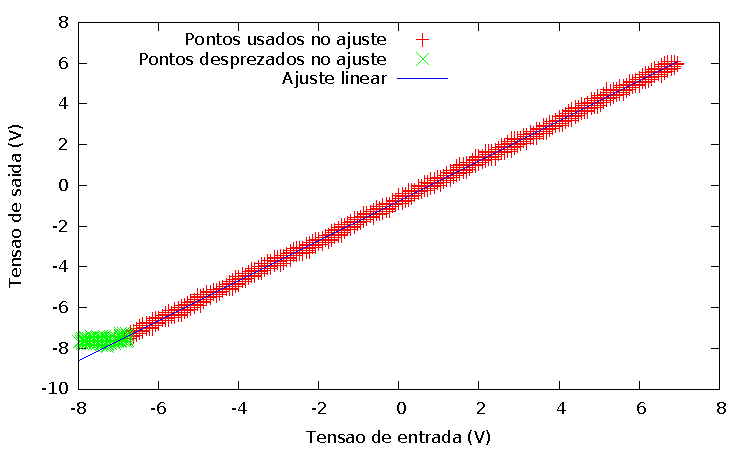
\includegraphics[width=3in]{v_rel.pdf}
\caption{Gráfico da relação entre tensão de entrada e de saída da montagem utilizada e respectivo ajuste linear. É possível observar que para valores de tensão de entrada muito negativa, começa a haver distorção.}
\label{fig:v_rel}
\end{figure}
Os resultados obtidos através do ajuste foram os seguintes: a=$G_v=0.96\pm0.01$, b=$-0.69\pm0.01$V.
Este resultado encontra-se de acordo com teoria, visto que está em concordância com a equação \ref{eq:g_v} e com o valor esperado de $G_v=1$. Nota-se também que a tensão mínima de saída é de cerca de $V_{o_{min}\approx7.8$, o que implicaria que a tensão de saturação do transístor seria de $V_{{CE}_{sat}}\approx0.2V$, o que está de acordo com as especificações do fabricante, que estipula que o valor máximo desta tensão não ultrapassa 1.1V.
Para a relação entre corrente de entrada e de saída do circuito também se realizou um ajuste linear semelhante ao realizado anteriormente para se obter o ganho de corrente, apresentado juntamente com os dados experimentais na figura \ref{fig:curr_rel}.
\begin{figure}
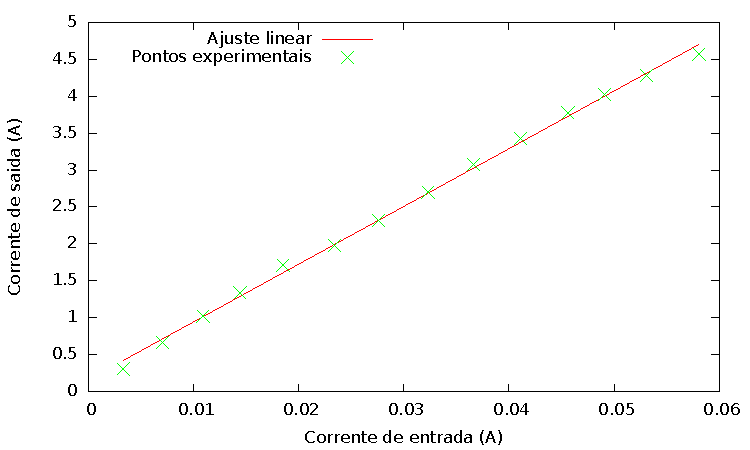
\includegraphics[width=3in]{curr_rel.pdf}
\caption{Gráfico da relação entre corrente de entrada e de saída da montagem utilizada e respectivo ajuste linear.}
\label{fig:curr_rel}
\end{figure}
Os resultados obtidos através do ajuste foram os seguintes: $a=G_i=78.12\pm1.07$, $b=0.16\pm0.04$A. A partir da equação \ref{eq:g_i} determinou-se que o ganho dos transístores utilizados era de $\beta_F=77.12$, estando este valor de acordo com as especificações do fabricante, que estipula que o ganho de corrente dos transístores é de cerca de 70.
\subsection{Potências fornecidas e dissipadas}
Os dados obtidos estão apresentados na tabela \ref{tab:fixe}:
% Please add the following required packages to your document preamble:
% \usepackage{multirow}
\begin{table}[h]
\begin{tabular}{|cc|c|c|}
                                                             & \multicolumn{1}{l|}{} & $v_o=v_{o_m}$ & $v_o=\frac{v_{o_m}}{2}$ \\ \hline
$V_{CC}$ (V)                                                 & \multicolumn{1}{l|}{} & \multicolumn{2}{c|}{8.04}               \\ \hline
$V_{DD}$ (V)                                                 & \multicolumn{1}{l|}{} & \multicolumn{2}{c|}{8.01}               \\ \hline
$I(V_{CC})$ (A)                                              & \multicolumn{1}{l|}{} & \multicolumn{2}{c|}{0.6}                \\ \hline
$I(V_{DD})$ (A)                                              & \multicolumn{1}{l|}{} & \multicolumn{2}{c|}{1.3}                \\ \hline
$R_L$ ($\Omega$)                                             &                       & \multicolumn{2}{c|}{10}                 \\ \hline
\multicolumn{1}{|c|}{\multirow{2}{*}{$V_o$ (V)}}             & multímetro            & -0.95         & -0.98                   \\ \cline{2-4} 
\multicolumn{1}{|c|}{}                                       & osciloscópio          & -0.93         & -0.95                   \\ \hline
\multicolumn{1}{|c|}{\multirow{2}{*}{$P_{Q_1}$ (W)}}         & multímetro            & 5.39          & 5.41                    \\ \cline{2-4} 
\multicolumn{1}{|c|}{}                                       & osciloscópio          & 5.38          & 5.39                    \\ \hline
\multicolumn{1}{|c|}{\multirow{2}{*}{$P_{Q_2}$ (W)}}         & multímetro            & 5.52          & 7.82                    \\ \cline{2-4} 
\multicolumn{1}{|c|}{}                                       & osciloscópio          & 5.52          & 7.81                    \\ \hline
\begin{tabular}[c]{@{}c@{}}Potência\\ dissipada\end{tabular} &                       & 10.89         & 13.2                    \\ \hline
\begin{tabular}[c]{@{}c@{}}Potência\\ fornecida\end{tabular} &                       & 15.24         & 15.24                   \\ \hline
Rendimento (\%)                                              &                       & 13.59         & 3.86                   
\end{tabular}
\caption{Tensões e potências dissipadas obtidas para os trasístores $Q_1$ e $Q_2$ da montagem utilizada.}
\label{tab:fixe}
\end{table}
É de notar que o rendimento obtido é bastante baixo, na ordem dos 15\% quando $v_o=v_{o_{max}}$ e na ordem dos 4\% quando $v_o=\frac{v_{o_m}}{2}$. É interessante notar que a eficiência obtida experimentalmente é bastante inferior à eficiência de 25\% obtida teoricamente. Isto deve-se ao facto de no cálculo da eficiência apenas se ter considerado as perdas nos transístores $Q_1$ e $Q_2$, quando existem outros elementos do circuito onde também existe dissipação.









\subsection{Impedâncias de entrada e saída}
Neste ponto mediram-se a tensão e corrente de entrada directamente utilizando o multímetro, de modo a determinar a impedância de entrada. Mediram-se também, utilizando duas cargas diferentes, a corrente e tensão nessas cargas, para que, a partir do equivalente de Thévenin fosse possível determinar a impedância de saída do circuito. Os resultados estão na tabela \ref{tab:impedancia}.

\begin{table}[h]
    \begin{tabular}{|l|l|}
\hline
          v_i (V)	&	$0.874  \pm 0.01$		                    \\ \hline
	i_i (A)	&	$0.00034 \pm 0.0001$			\\ \hline 
	R_1 ($\Omega$) &	$10\pm0.1$			 \\ \hline
	v_{01} (V)	&   	$0.851\pm0.01$	                       \\ \hline
           R_2 ($\Omega$) &  $8\pm0.1$   \\ \hline
           v_{02} (V) &   $0.835 \pm 0.01$ \\ \hline

    \end{tabular}
\end{table}






















\subsection{Resposta em frequência}






%%%%%%%%%%%%%%%%%%%%%%%%%%% Análise dos resultados %%%%%%%%%%%%%%%%%%%%%%%%%%%%%
\section{Análise de resultados}
\label{s:aresul}
\subsection{Ponto de funcionamento em repouso}
\subsection{Função de transferência}
\subsection{Potências fornecidas e dissipadas}
\subsection{Impedâncias de entrada e saída}
\subsection{Resposta em frequência}


%%%%%%%%%%%%%%%%%%%%%%%%%%% Conclusões e Críticas %%%%%%%%%%%%%%%%%%%%%%%%%%%%%%
\section{Conclusões e Críticas}
\label{s:conclu}
%Incluir melhorias propostas à experiência


%\begin{acknowledgments}
%\end{acknowledgments}

%%%%%%%%%%%%%%%%%%%%%%%%%%%%%%%%%%%%%%%%%%%%%%%%%%%%%%%%%%%%%%%%%%%%%%%%%%%%%%%%
% % % % % % % % % % % % % % % %     FIM    % % % % % % % % % % % % % % % % % % % 
%%%%%%%%%%%%%%%%%%%%%%%%%%%%%%%%%%%%%%%%%%%%%%%%%%%%%%%%%%%%%%%%%%%%%%%%%%%%%%%%

\nocite{*}
\bibliography{bibliografia}{}
\bibliographystyle{plain}% Produces the bibliography via BibTeX.
\end{document}
%end of file
